C\# ist eine objektorientierte Programmiersprache, die im Auftrag von Microsoft entwickelt wurde und die es bereits seit 2001 gibt. In der Abbildung seht ihr das Logo der Programmiersprache. 

\begin{figure}[H]
	\caption{Das Logo der Programmiersprache C\#}
	\centering
	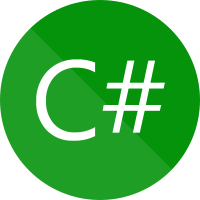
\includegraphics[width=2cm]{exercises/references/csharp.png}
\end{figure}

Das nachstehende Quelltext-Listing zeigt ein Programm, das den Text \enquote{Hello LaTeX friends!} auf der Konsole ausgibt. Ähnlich wie bei Java werden auch in C\# Klassen und eine Main-Methode verwendet, um eine ausführbare Anwendung zu bauen. 

\inputminted[breaklines, linenos=true]{csharp}{exercises/references/HelloLateXFriends.cs}




